% This is text associated with the open textbook "Open Electromagnetics"
% See immediately below for author, date
% This work is licensed under the Creative Commons Attribution-ShareAlike 4.0 International License. (CC BY-SA 4.0) 
% To view a copy of the license, visit http://creativecommons.org/licenses/by-sa/4.0/

%ORB TITLE Cylindrical Coordinates
%ORB AUTHOR 0        # S.W. Ellingson, Virginia Tech (ellingson@vt.edu)
%ORB DATE 20180803   # yyyymmdd
%ORB ABSTRACT Cylindrical Coordinates

\label{m0096_Cylindrical_Coordinates} % <-- Must match name of this file and module directory name.  Don't mess with this!
\index{cylindrical coordinate system|(}

Cartesian coordinates (Section~\ref{m0004_Cartesian_Coordinates}) are not convenient in certain cases.  
One of these is when the problem has cylindrical symmetry.
For example, in the Cartesian coordinate system, the cross-section of a cylinder concentric with the $z$-axis requires two coordinates to describe: $x$ and $y$.
However, this cross section can be described using a single parameter -- namely the radius -- which is $\rho$ in the cylindrical coordinate system.
This results in a dramatic simplification of the mathematics in some applications.

The cylindrical system is defined with respect to the Cartesian system in Figure~\ref{m0096_fCylindricalCoordinates}.
In lieu of $x$ and $y$, the cylindrical system uses $\rho$, the distance measured from the closest point on the $z$ axis,\footnote{Note that some textbooks use ``$r$'' in lieu of $\rho$ for this coordinate.} and $\phi$, the angle measured in a plane of constant $z$, beginning at the $+x$ axis ($\phi=0$) with $\phi$ increasing toward the $+y$ direction.
%
\begin{figure}[b!]
\begin{center}
\pdftooltip{{  % note double braces
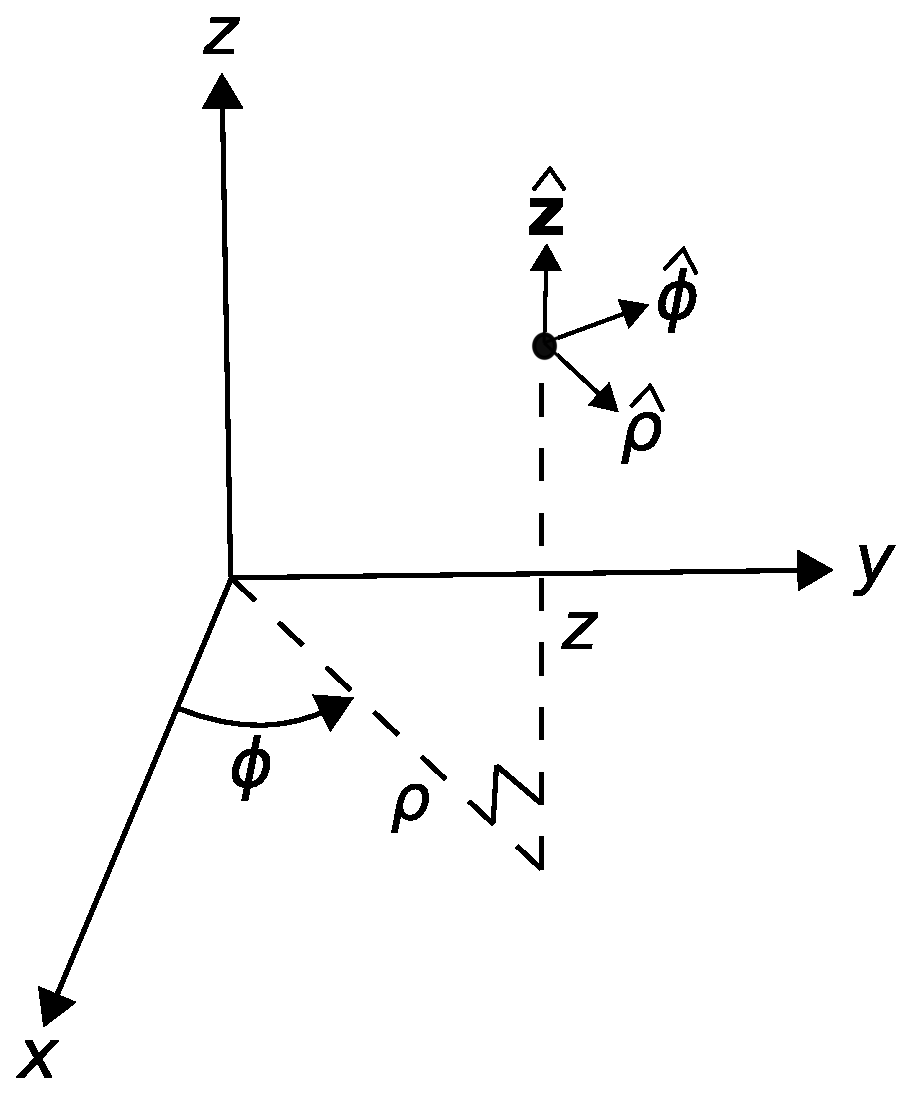
\includegraphics[width=2in]{modules/m0096_fCylindricalCoordinates.eps}
% https://commons.wikimedia.org/wiki/File:M0096_fCylindricalCoordinates.svg
}}{Cartesian coordinate system with a point arbitrarily plotted in the positive x, y, and z axes. A dashed line in the xy-plane labeled rho indicates the point’s distance from the z-axis and is shown at an angle phi from the x-axis. Another dashed line labeled z is perpendicular to rho, extends vertically from the xy-plane, and connects to the plotted point. The point has vector z-hat pointed in the z-direction. rho-hat points away from the origin, parallel to rho. phi-hat is perpendicular to z-hat and rho-hat.}
\end{center} 
\centerline{\scriptsize 
\copyright~\hyperref[m0096_fCylindricalCoordinates_Credit]{K.\ Kikkeri} 
\href{https://creativecommons.org/licenses/by-sa/4.0/}{CC BY~SA 4.0} 
} 
\caption{
\label{m0096_fCylindricalCoordinates}
Cylindrical coordinate system and associated basis vectors.
}
\end{figure}

The basis vectors in the cylindrical system are $\hat{\bf \rho}$, $\hat{\bf \phi}$, and $\hat{\bf z}$.
As in the Cartesian system, the dot product of like basis vectors is equal to one, and the dot product of unlike basis vectors is equal to zero.
The cross products of basis vectors are as follows:
%
\begin{equation}
\hat{\bf \rho} \times \hat{\bf \phi} = \hat{\bf z}
\end{equation}
%
\begin{equation}
\hat{\bf \phi} \times \hat{\bf z} = \hat{\bf \rho}
\end{equation}
%
\begin{equation}
\hat{\bf z} \times \hat{\bf \rho} = \hat{\bf \phi}
\end{equation}
%
A useful diagram that summarizes these relationships is shown in Figure~\ref{m0096_fCylindricalBasisCrossProducts}.
%
\begin{figure}
\begin{center}
\pdftooltip{{  % note double braces
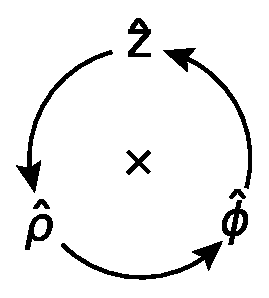
\includegraphics[width=1in]{modules/m0096_fCylindricalBasisCrossProducts.eps}
}}{The symbols for rho-hat, phi-hat, and z-hat are arranged in a circle, connected by arrows pointing in a counter-clockwise direction.  A cross product symbol appears in the center of the circle.}
\end{center} 
\caption{\label{m0096_fCylindricalBasisCrossProducts}Cross products among basis vectors in the cylindrical system. (See Figure~\ref{m0006_fCartesianBasisCrossProducts} for instructions on the use of this diagram.)}
\end{figure}

The cylindrical system is usually less useful than the Cartesian system for identifying absolute and relative positions.
This is because the basis directions depend on position.
For example, $\hat{\bf \rho}$ is directed radially outward from the $\hat{\bf z}$ axis, so $\hat{\bf \rho}=\hat{\bf x}$ for locations along the $x$-axis but $\hat{\bf \rho}=\hat{\bf y}$ for locations along the $y$ axis.
Similarly, the direction $\hat{\bf \phi}$ varies as a function of position.
To overcome this awkwardness, it is common to set up a problem in cylindrical coordinates in order to exploit cylindrical symmetry, but at some point to convert to Cartesian coordinates.  
Here are the conversions:
%
\begin{equation}
x = \rho\cos\phi
\end{equation}
%
\begin{equation}
y = \rho\sin\phi
\end{equation}
%
and $z$ is identical in both systems.  The conversion from Cartesian to cylindrical is as follows:
%
\begin{equation}
\rho = \sqrt{x^2+y^2}
\end{equation}
%
\begin{equation}
\phi = \arctan\left(y,x\right)
\end{equation}
%
where $\arctan$ is the \emph{four-quadrant} inverse tangent function; i.e., $\arctan(y/x)$ in the first quadrant ($x>0$, $y>0$), but possibly requiring an adjustment for the other quadrants because the signs of both $x$ and $y$ are individually significant.\footnote{Note that this function is available in MATLAB and Octave as {\tt atan2(y,x)}.}

Similarly, it is often necessary to represent basis vectors of the cylindrical system in terms of Cartesian basis vectors and vice-versa.
Conversion of basis vectors is straightforward using dot products to determine the components of the basis vectors in the new system. 
For example, $\hat{\bf x}$ in terms of the basis vectors of the cylindrical system is
%
\begin{equation}
\hat{\bf x} = \hat{\bf \rho}\left(\hat{\bf \rho}\cdot\hat{\bf x}\right) 
             +\hat{\bf \phi}\left(\hat{\bf \phi}\cdot\hat{\bf x}\right)
             +\hat{\bf z   }\left(\hat{\bf    z}\cdot\hat{\bf x}\right)
\end{equation}
%
The last term is of course zero since $\hat{\bf z}\cdot\hat{\bf x}=0$.
Calculation of the remaining terms requires dot products between basis vectors in the two systems, which are summarized in Table~\ref{m0096_tBasisVectorConversion}.
Using this table, we find
%
\begin{equation}
\hat{\bf x} = \hat{\bf \rho}\cos\phi
             -\hat{\bf \phi}\sin\phi
\end{equation}
%
\begin{equation}
\hat{\bf y} = \hat{\bf \rho}\sin\phi
             +\hat{\bf \phi}\cos\phi
\end{equation}
%
and of course $\hat{\bf z}$ requires no conversion.  Going from Cartesian to cylindrical, we find
%
\begin{equation}
\hat{\bf \rho} = \hat{\bf x}\cos\phi
                +\hat{\bf y}\sin\phi
\end{equation}
%
\begin{equation}
\hat{\bf \phi} =-\hat{\bf x}\sin\phi
                +\hat{\bf y}\cos\phi
\end{equation}
%
\begin{table}
\begin{center}
\begin{tabular}{c|ccc}
$\cdot$       & $\hat{\bf \rho}$ & $\hat{\bf \phi}$ & $\hat{\bf z}$ \\
\hline
$\hat{\bf x}$ & $\cos\phi$       & $-\sin\phi$      & 0 \\
$\hat{\bf y}$ & $\sin\phi$       & $~\cos\phi$      & 0 \\
$\hat{\bf z}$ & 0              & 0              & 1 \\
\end{tabular}
\end{center}
\caption{\label{m0096_tBasisVectorConversion}Dot products between basis vectors in the cylindrical and Cartesian coordinate systems.}
\end{table}

{\bf Integration Over Length.}  
A differential-length segment of a curve in the cylindrical system is described in general as
%
\begin{equation}
d{\bf l} = \hat{\bf \rho}d\rho + \hat{\bf \phi}\rho d\phi + \hat{\bf z}~dz 
\end{equation}
%
Note that the contribution of the $\phi$ coordinate to differential length is $\rho d\phi$, not simply $d\phi$.
This is because $\phi$ is an angle, not a distance. 
To see why the associated distance is $\rho d\phi$, consider the following.
The circumference of a circle of radius $\rho$ is $2\pi\rho$.  
If only a fraction of the circumference is traversed, the associated arclength is the circumference scaled by $\phi/2\pi$, where $\phi$ is the angle formed by the traversed circumference.
Therefore, the distance is $2\pi\rho \cdot \phi/2\pi = \rho \phi$, and the differential distance is $\rho d\phi$. 

As always, the integral of a vector field ${\bf A}({\bf r})$ over a curve ${\mathcal C}$ is
%
\begin{equation}
\int_{\mathcal C}{ {\bf A}\cdot d{\bf l} }
\end{equation}
%
To demonstrate the cylindrical system, let us calculate the integral of ${\bf A}({\bf r})=\hat{\bf \phi}$ when $\mathcal{C}$ is a circle of radius $\rho_0$ in the $z=0$ plane, as shown in Figure~\ref{m0096_Circle}.  In this example, 
$d{\bf l} = \hat{\bf \phi}~\rho_0~d\phi$ since $\rho=\rho_0$ and $z=0$ are both constant along ${\mathcal C}$.  Subsequently, ${\bf A}\cdot d{\bf l}=\rho_0 d\phi$ and the above integral is
%
\begin{equation}
\int_{0}^{2\pi}{ \rho_0~d\phi } = 2\pi\rho_0
\end{equation}
%
i.e., this is a calculation of circumference.
%
\begin{figure}
\begin{center}
\pdftooltip{{  % note double braces
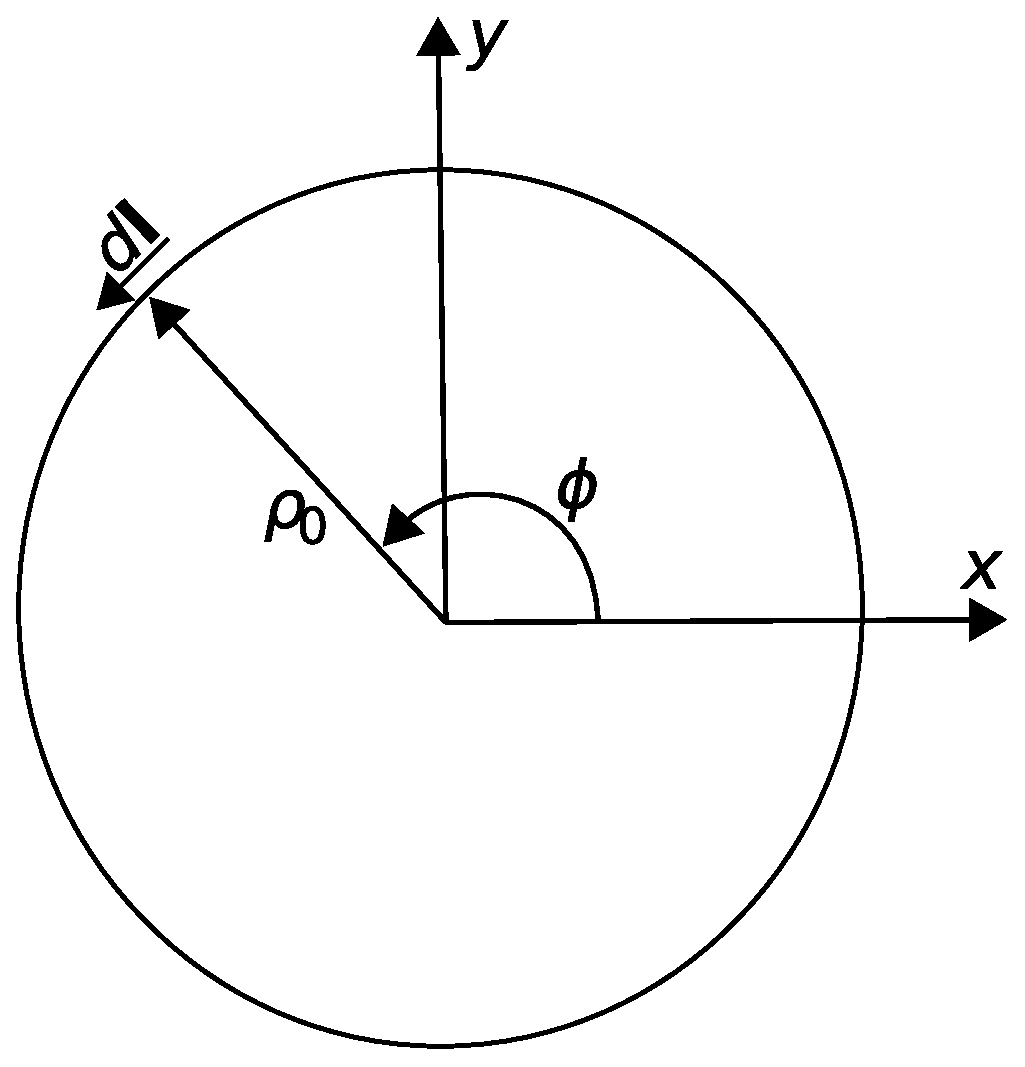
\includegraphics[width=2in]{modules/m0096_Circle.eps}
% https://commons.wikimedia.org/wiki/File:Cylindrical_Coordinates_Example.svg
}}{A circle lies in the traditional xy-plane with its center at the origin. Radius rho sub 0 is represented as a vector in the second quadrant of the coordinate system. phi represents the angle formed by the positive x-axis and rho sub 0. d vector l runs counterclockwise around the circumference of the circle.}
\end{center} 
\centerline{\scriptsize 
\copyright~\hyperref[m0096_Circle_Credit]{K.\ Kikkeri} 
\href{https://creativecommons.org/licenses/by-sa/4.0/}{CC BY~SA 4.0} 
} 
\caption{
\label{m0096_Circle}
Example in cylindrical coordinates: The circumference of a circle.
}
\end{figure}

Note that the cylindrical system is an appropriate choice for the preceding example because the problem can be expressed with the minimum number of varying coordinates in the cylindrical system.
If we had attempted this problem in the Cartesian system, we would find that both $x$ and $y$ vary over ${\mathcal C}$, and in a relatively complex way.\footnote{Nothing will drive this point home more firmly than trying it.  It can be done, but it's a lot more work...}

{\bf Integration Over Area.}  
Now we ask the question, what is the integral of some vector field ${\bf A}$ over a circular surface ${\mathcal S}$ in the $z=0$ plane having radius $\rho_0$? 
This is shown in Figure~\ref{m0096_CircleArea}.
The differential surface vector in this case is
%
\begin{equation}
d{\bf s} = \hat{\bf z}~\left( d\rho \right) \left( \rho d\phi \right) = \hat{\bf z}~\rho~d\rho~d\phi  
\end{equation}
%
The quantities in parentheses are the radial and angular dimensions, respectively.
The direction of $d{\bf s}$ indicates the direction of positive flux 
\index{flux}
-- see the discussion in Section~\ref{m0004_Cartesian_Coordinates} for an explanation.  
In general, the integral over a surface is
%
\begin{equation}
\int_{\mathcal S} {\bf A}\cdot d{\bf s}
\end{equation}
%
To demonstrate, let's consider ${\bf A}=\hat{\bf z}$; in this case ${\bf A}\cdot d{\bf s} = \rho~d\rho~d\phi$ and the integral becomes
%
\begin{equation}
\begin{split}
\int_{0}^{\rho_0}\int_{0}^{2\pi} \rho~d\rho~d\phi &= \left( \int_{0}^{\rho_0} \rho~d\rho \right) \left( \int_{0}^{2\pi} d\phi \right) \\
                                                  &= \left( \frac{1}{2}\rho_0^2 \right) \left( 2\pi \right) \\
                                                  &= \pi \rho_0^2
\end{split}
\end{equation}
%
which we recognize as the area of the circle, as expected.
The corresponding calculation in the Cartesian system is quite difficult in comparison.
%
\begin{figure}
\begin{center}
\pdftooltip{{  % note double braces
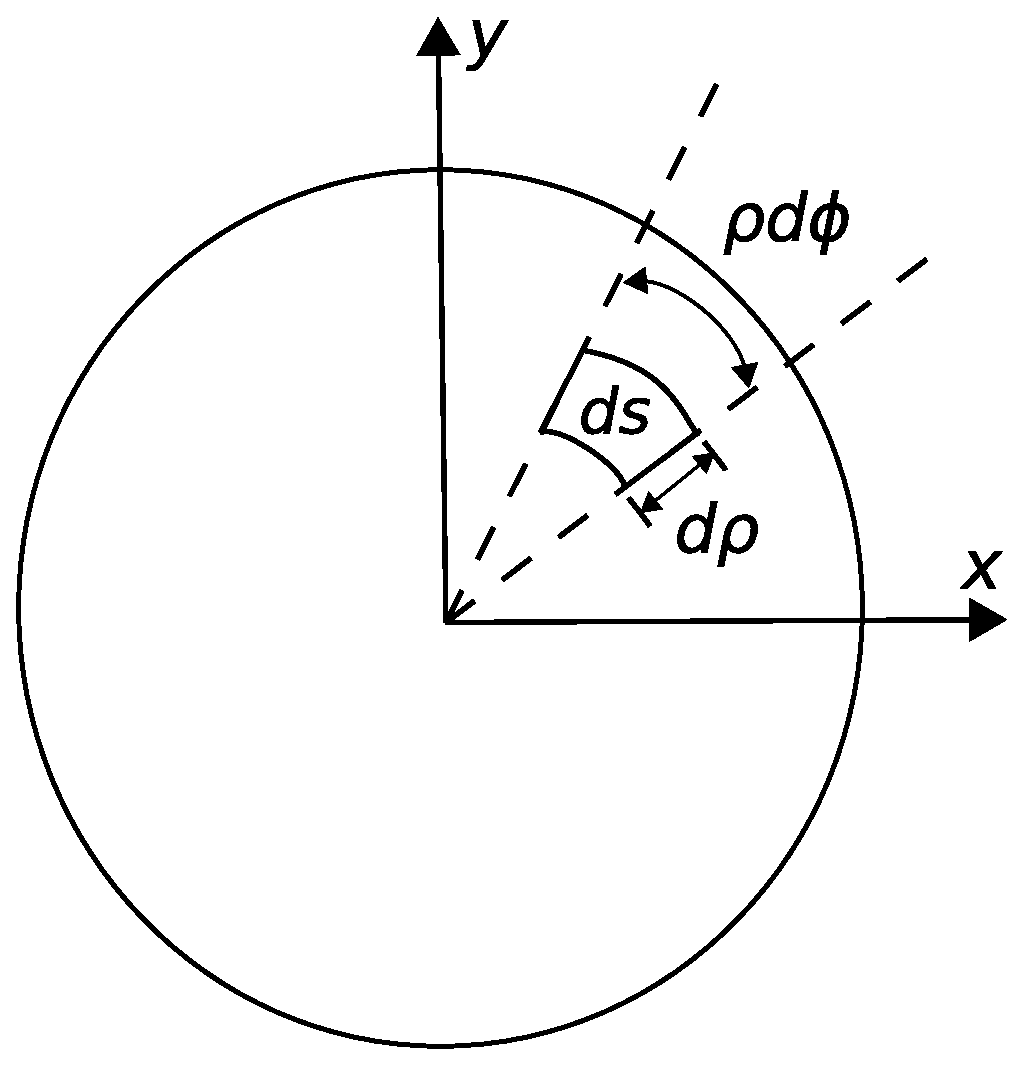
\includegraphics[width=2in]{modules/m0096_CircleArea.eps}
% https://commons.wikimedia.org/wiki/File:Cylindrical_Coordinates-Area_of_a_Circle.svg
}}{A circle in the xy-plane with its center at the origin. Two dashed lines emanate from the center of the circle to form an acute angle in the first quadrant of the circle. The section of the circumference blocked off by these two dashed lines is labeled rho * d phi. A section of the radius along one of the dashed lines is labeled d rho. This section of the radius is swept in the radial direction to the other dashed line to form a section of area called ds.}
\end{center} 
\centerline{\scriptsize 
\copyright~\hyperref[m0096_CircleArea_Credit]{K.\ Kikkeri} 
\href{https://creativecommons.org/licenses/by-sa/4.0/}{CC BY~SA 4.0} 
} 
\caption{
\label{m0096_CircleArea}
Example in cylindrical coordinates: The area of a circle.
}
\end{figure}

Whereas the previous example considered a planar surface, we might consider instead a curved surface.
Here we go.
What is the integral of a vector field ${\bf A}=\hat{\bf \rho}$ over a cylindrical surface ${\mathcal S}$ concentric with the $z$ axis having radius $\rho_0$ and extending from $z=z_1$ to $z=z_2$? 
This is shown in Figure~\ref{m0096_CylinderArea}.
%
\begin{figure}
\begin{center}
\pdftooltip{{  % note double braces
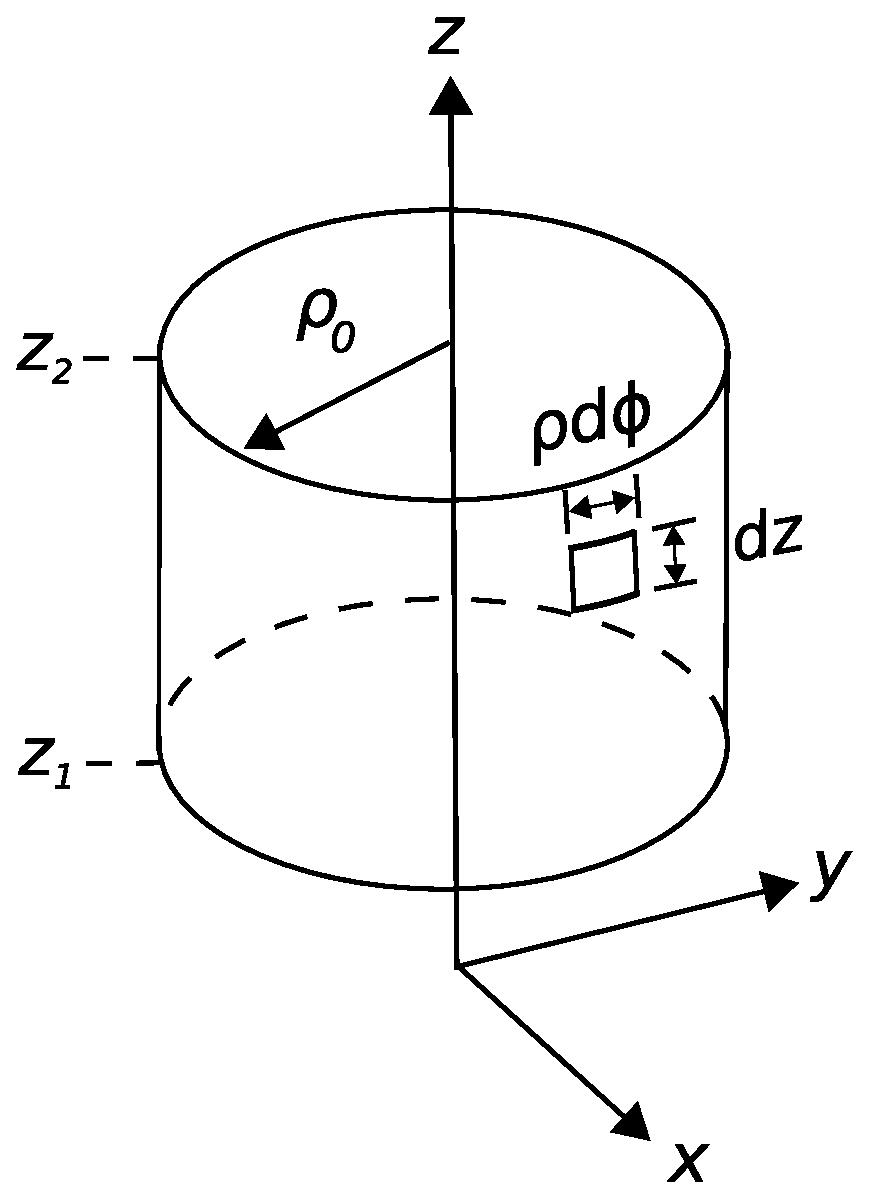
\includegraphics[width=2in]{modules/m0096_CylinderArea.eps}
% https://commons.wikimedia.org/wiki/File:M0096_CylinderArea.svg
}}{A cylinder lies in a Cartesian coordinate system with its centerline coincident with the positive z-axis. The height of the bottom surface of the cylinder is labeled z sub 1 and the height of the top surface is labeled z sub 2. The radius of the cylinder is labeled rho sub zero. An arbitrary section of the surface is described in width as rho d phi with height dz.}
\end{center} 
\centerline{\scriptsize 
\copyright~\hyperref[m0096_CylinderArea_Credit]{K.\ Kikkeri} 
\href{https://creativecommons.org/licenses/by-sa/4.0/}{CC BY~SA 4.0} 
} 
\caption{
\label{m0096_CylinderArea}
Example in cylindrical coordinates: The area of the curved surface of a cylinder.
}
\end{figure}
%
The differential surface vector in this case is
%
\begin{equation}
d{\bf s} = \hat{\bf \rho}\left( \rho_0 d\phi \right) \left( dz \right) = \hat{\bf \rho}\rho_0~d\phi~dz
\end{equation}
%
The integral is
%
\begin{equation}
\begin{split}
\int_{\mathcal S} {\bf A}\cdot d{\bf s} &= \int_{0}^{2\pi}\int_{z_1}^{z_2} \rho_0~d\phi dz \\
                                        &= \rho_0 \left( \int_{0}^{2\pi} d\phi \right) \left( \int_{z_1}^{z_2} dz \right)\\
                                        &= 2\pi \rho_0 \left(z_2-z_1\right) \\
\end{split}
\end{equation}
%
which is the area of ${\mathcal S}$, as expected.
Once again, the corresponding calculation in the Cartesian system is quite difficult in comparison.


{\bf Integration Over Volume.}  
The differential volume element in the cylindrical system is
%
\begin{equation}
dv ~=~ d\rho~\left(\rho d\phi\right)~dz ~=~ \rho~d\rho~d\phi~dz
\end{equation}

For example, if $A({\bf r})=1$ and the volume $\mathcal{V}$ is a cylinder bounded by $\rho\le \rho_0$ and $z_1\le z \le z_2$, then 
%
\begin{equation}
\begin{split}
\int_{\mathcal V} A({\bf r})~dv  &= \int_{0}^{\rho_0} \int_{0}^{2\pi} \int_{z_1}^{z_2} \rho~d\rho~d\phi~dz \\
                                 &= \left(\int_{0}^{\rho_0} \rho~d\rho \right)  \left( \int_{0}^{2\pi} d\phi \right)  \left( \int_{z_1}^{z_2} dz\right) \\
                                 & = \pi \rho_0^2 \left(z_2-z_1\right) 
\end{split}
\end{equation} 
%
i.e., area times length, which is volume.

Once again, the procedure above is clearly more complicated than is necessary if we are interested only in computing volume.
However, if the integrand is not constant-valued then we are no longer simply computing volume.
In this case, the formalism is appropriate and possibly necessary.  

%%%%%%%%%%%%%%%%%%%%%%%%%%%%%%%%%%%%

{\bf Additional Reading:}
\begin{itemize}
\item ``\href{https://en.wikipedia.org/wiki/Cylindrical_coordinate_system}{Cylindrical coordinate system}'' on Wikipedia.
\end{itemize}

\index{cylindrical coordinate system|)}
